%----------------------------------------------------------
% DREAM PhD Timeline: WP1-5 distributed over 3 years
% Shows sequencing, de-risking, and critical decision points
%----------------------------------------------------------

\begin{figure}[H]
    \centering
    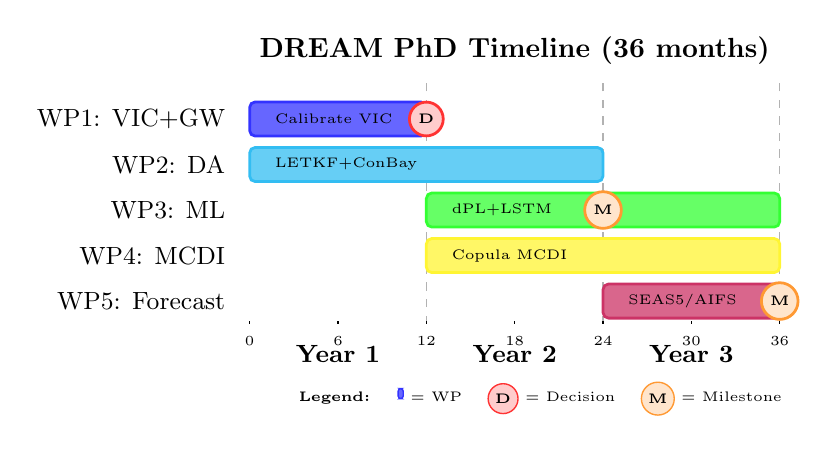
\begin{tikzpicture}[
        scale=0.85,
        x=0.22cm,  % 1 month = 0.22cm
        y=0.85cm,  % each WP row = 0.85cm
    ]

    % Title
    \node[anchor=north, font=\bfseries\normalsize, yshift=0.3cm] at (18, 5.5) {DREAM PhD Timeline (36 months)};

    % Y-axis labels (WP)
    \node[anchor=east, font=\small] at (-1.0, 4.3) {WP1: VIC+GW};
    \node[anchor=east, font=\small] at (-1.0, 3.5) {WP2: DA};
    \node[anchor=east, font=\small] at (-1.0, 2.7) {WP3: ML};
    \node[anchor=east, font=\small] at (-1.0, 1.9) {WP4: MCDI};
    \node[anchor=east, font=\small] at (-1.0, 1.1) {WP5: Forecast};

    % Year separators (vertical dashed lines at 12, 24, 36 months)
    \foreach \month in {12, 24, 36} {
        \draw[dashed, gray!60, line width=0.5pt] (\month, 0.7) -- (\month, 5.0);
    }

    % X-axis year labels
    \node[anchor=north, font=\bfseries\small] at (6, 0.5) {Year 1};
    \node[anchor=north, font=\bfseries\small] at (18, 0.5) {Year 2};
    \node[anchor=north, font=\bfseries\small] at (30, 0.5) {Year 3};

    % WP1: Full Year 1
    \draw[fill=blue!60, draw=blue!80, line width=1pt, rounded corners=2pt] (0, 4.0) rectangle (12, 4.6);
    \node[anchor=west, font=\tiny, xshift=3pt] at (0.5, 4.3) {Calibrate VIC};

    % Decision marker at month 12
    \node[anchor=center, draw=red!80, fill=red!20, circle, inner sep=2pt, font=\tiny\bfseries, line width=1pt] at (12, 4.3) {D};

    % WP2: Months 0–24
    \draw[fill=cyan!60, draw=cyan!80, line width=1pt, rounded corners=2pt] (0, 3.2) rectangle (24, 3.8);
    \node[anchor=west, font=\tiny, xshift=3pt] at (0.5, 3.5) {LETKF+ConBay};

    % WP3: Months 12–36
    \draw[fill=green!60, draw=green!80, line width=1pt, rounded corners=2pt] (12, 2.4) rectangle (36, 3.0);
    \node[anchor=west, font=\tiny, xshift=3pt] at (12.5, 2.7) {dPL+LSTM};

    % Milestone at month 24
    \node[anchor=center, draw=orange!80, fill=orange!20, circle, inner sep=2pt, font=\tiny\bfseries, line width=1pt] at (24, 2.7) {M};

    % WP4: Months 12–36
    \draw[fill=yellow!60, draw=yellow!80, line width=1pt, rounded corners=2pt] (12, 1.6) rectangle (36, 2.2);
    \node[anchor=west, font=\tiny, xshift=3pt] at (12.5, 1.9) {Copula MCDI};

    % WP5: Months 24–36
    \draw[fill=purple!60, draw=purple!80, line width=1pt, rounded corners=2pt] (24, 0.8) rectangle (36, 1.4);
    \node[anchor=west, font=\tiny, xshift=3pt] at (24.5, 1.1) {SEAS5/AIFS};

    % Final milestone at month 36
    \node[anchor=center, draw=orange!80, fill=orange!20, circle, inner sep=2pt, font=\tiny\bfseries, line width=1pt] at (36, 1.1) {M};

    % Month ticks (every 6 months)
    \foreach \month in {0, 6, 12, 18, 24, 30, 36} {
        \draw[line width=0.5pt] (\month, 0.7) -- (\month, 0.75);
        \node[anchor=north, font=\tiny] at (\month, 0.65) {\month};
    }

    % Legend box
    \node[anchor=west, font=\tiny, xshift=0.5cm, yshift=-0.3cm] at (0, -0.2) {
        \textbf{Legend:} \quad
        \tikz[baseline=-0.15em]{\draw[fill=blue!60, draw=blue!80, rounded corners=1pt, line width=0.5pt] (0,0) rectangle (0.3,0.15);} = WP
        \quad
        \tikz[baseline=-0.15em]{\node[draw=red!80, fill=red!20, circle, inner sep=1.5pt, font=\tiny\bfseries, line width=0.5pt] {D};} = Decision
        \quad
        \tikz[baseline=-0.15em]{\node[draw=orange!80, fill=orange!20, circle, inner sep=1.5pt, font=\tiny\bfseries, line width=0.5pt] {M};} = Milestone
    };

    \end{tikzpicture}
    \caption{%
        DREAM PhD timeline showing five interconnected work packages over 36 months.
        \textbf{WP1} establishes a physics-based VIC-Denmark baseline with groundwater coupling (Year 1), followed by a critical decision (D) on 2D lateral coupling.
        \textbf{WP2} (LETKF + ConBay data assimilation) runs in parallel throughout, constraining all physical parameters.
        \textbf{WP3} (differentiable hydrology + LSTM hybrid) and \textbf{WP4} (copula-aggregated multi-pillar drought index) execute in Years 2--3 in parallel.
        \textbf{WP5} (SEAS5/AIFS seasonal forecasting) focuses on Year 3 outputs.
        The timeline demonstrates de-risking: Year 1 alone delivers a publishable physics baseline even if hybrid extensions slip.
        Milestones (M) mark completion of hybrid competence (month 24) and operational prototype readiness (month 36).
    }
    \label{fig:timeline}
\end{figure}
